\chapter{\LaTeX の基本}
	\section{参考文献の引用方法}
	参考文献を論文中で引用するときはref.bibファイルに参考文献情報を貼り付けたうえで次のように引用しましょう\cite{G_ng_r_2021}.
	\section{数式について}
	文中式は $\hat{g}_{\mu\nu}=e^{2\omega}g_{\mu\nu}$ と書けます.その他別行立ての数式は次のような数式環境を用いて入力します.

	よく使用する数式については,./documents/define\_equations.texに,newcommandでマクロを定義しておくと便利です.
		\begin{equation}
			R_{\mu\alpha\nu}^{\lambda}=\Riemanntensor{\lambda}{\mu}{\alpha}{\nu}{\sigma}\label{eq:Riemann_tensor}
		\end{equation}

	また,複数行にわたる数式変形をきれいに出力したいときは,dmath環境を用いると便利です.dmath環境では数式を自動で改行したり,等号の位置を自動で揃えてくれます.
		\begin{dmath}
			R_{rr} = \partial_{\lambda}\chr{\lambda}{r}{r}
			- \partial_{r}\chr{\lambda}{\lambda}{r}
			+ \chr{\lambda}{\lambda}{\ell}\chr{\ell}{r}{r}
			- \chr{\lambda}{r}{\ell}\chr{\ell}{\lambda}{r}
			= \qty{\partial_{t}\chr{t}{r}{r} - \partial_{r}\chr{t}{t}{r} + \chr{t}{t}{\ell}\chr{\ell}{r}{r} - \chr{t}{r}{\ell}\chr{\ell}{t}{r}}
			+ \qty{\partial_{\theta}\chr{\theta}{r}{r} - \partial_{r}\chr{\theta}{\theta}{r} + \chr{\theta}{\theta}{\ell}\chr{\ell}{r}{r} - \chr{\theta}{r}{\ell}\chr{\ell}{\theta}{r}}
			+ \qty{\partial_{\varphi}\chr{\varphi}{r}{r} - \partial_{r}\chr{\varphi}{\varphi}{r} + \chr{\varphi}{\varphi}{\ell}\chr{\ell}{r}{r} - \chr{\varphi}{r}{\ell}\chr{\ell}{\varphi}{r}} \nonumber \\
			= \qty{\partial_{t}\chr{t}{r}{r} - \chr{t}{r}{r}\chr{r}{t}{r}}
			+ \qty{- \partial_{r}\chr{\theta}{\theta}{r} + \chr{\theta}{\theta}{t}\chr{t}{r}{r} + \chr{\theta}{\theta}{r}\chr{r}{r}{r} - \chr{\theta}{r}{\theta}\chr{\theta}{\theta}{r}}
			+ \qty{- \partial_{r}\chr{\varphi}{\varphi}{r} + \chr{\varphi}{\varphi}{t}\chr{t}{r}{r} + \chr{\varphi}{\varphi}{r}\chr{r}{r}{r} - \chr{\varphi}{r}{\varphi}\chr{\varphi}{\varphi}{r}} \nonumber \\
			= \frac{\dot{a}^2+a\ddot a}{1-Kr^2} - \frac{a\dot a}{1-Kr^2}\frac{\dot a}{a} + \frac{1}{r^2} + \frac{\dot a}{a}\frac{a\dot a}{1-Kr^2} + \frac{1}{r}\frac{Kr}{1-Kr^2} + \frac{\dot a}{a}\frac{a\dot a}{1-Kr^2} + \frac{1}{r}\frac{Kr}{1-Kr^2} -\frac{1}{r^2} \nonumber \\
			= \frac{2\dot{a}^2+a\ddot a + 2K}{1-Kr^2}\label{eq:Ricci_tensor}
		\end{dmath}

	論文中の数式を引用したい場合は,引用したい数式にラベルを付け,引用したい箇所で「\textbackslash cref\{eq:作成したラベル\}」と入力すれば\cref{eq:Ricci_tensor}のように引用が可能です.数式ラベル内にeq:とつけているのは数式をエディタの検索機能や補完機能を利用しやすくするためです.

	その他,数式を入力する際には,physicsパッケージを用いるのが便利です(usepackageしてあります).

	\section{図の挿入と引用}
	図は以下のように挿入できます.
		\begin{figure}[htbp]
			\centering
			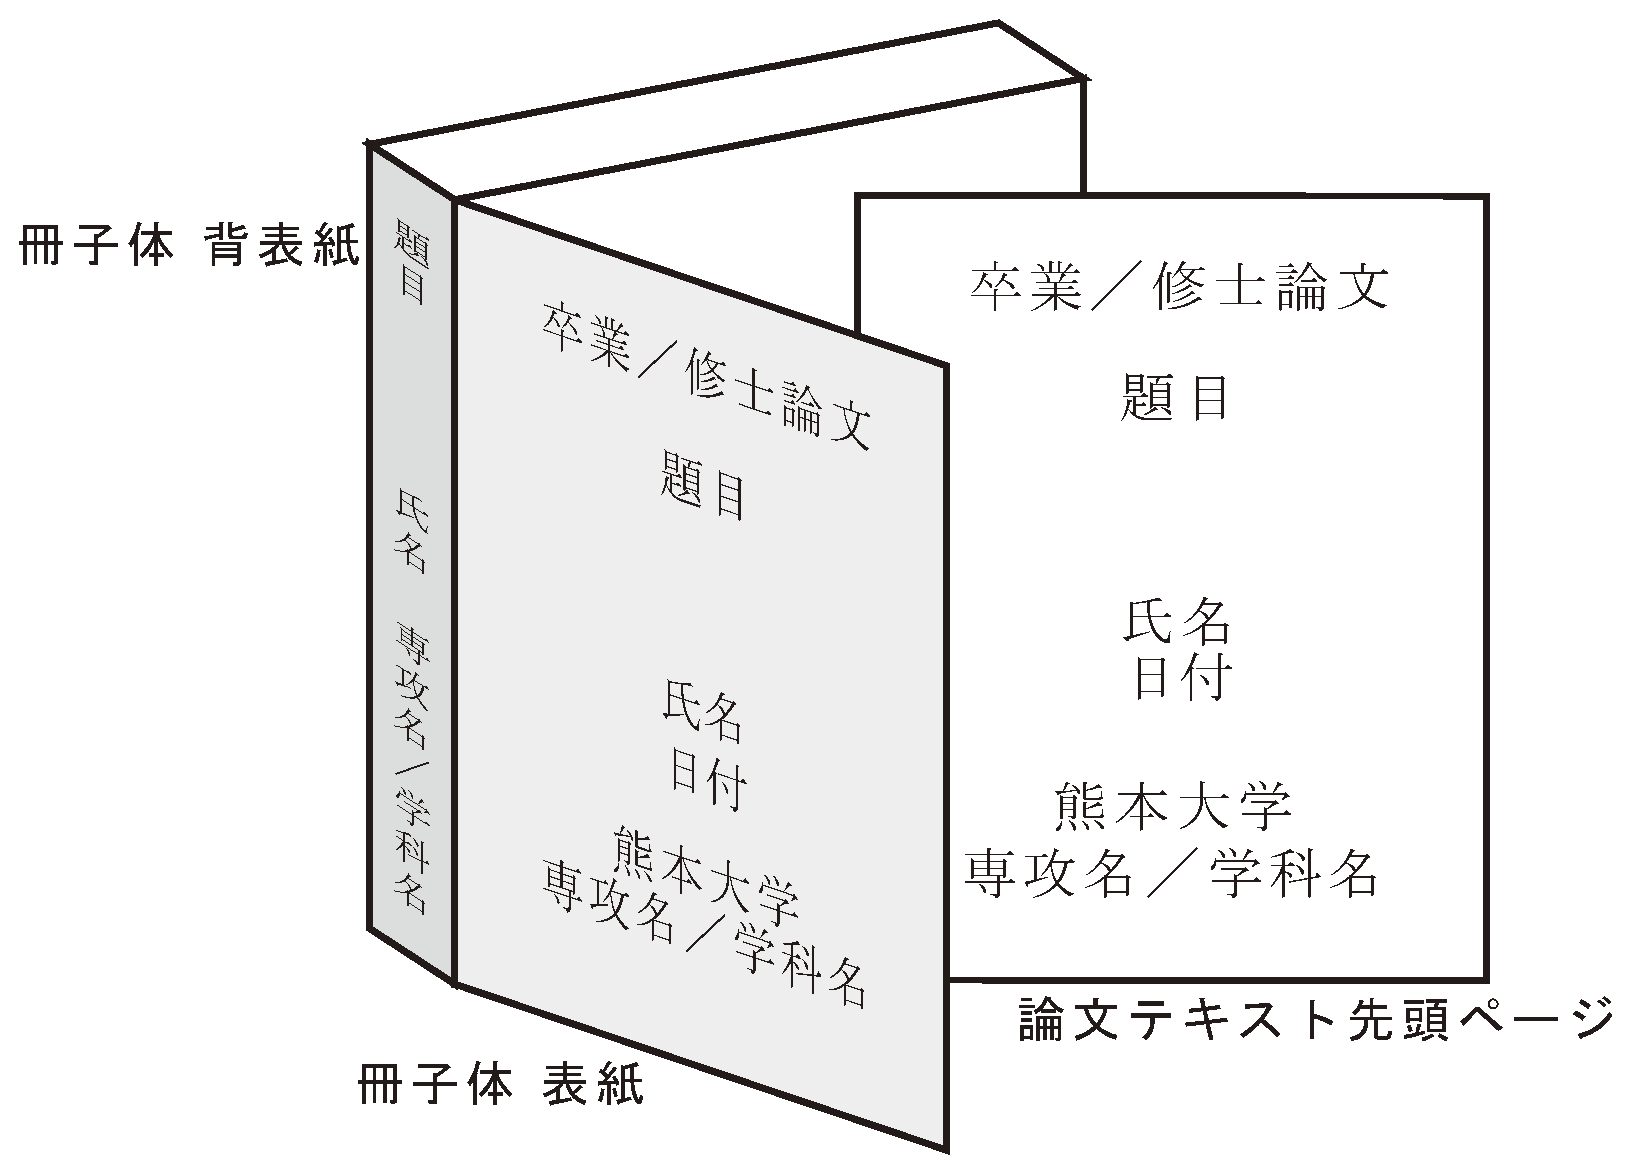
\includegraphics[width=1.0\linewidth,keepaspectratio]{./images/book.eps}
			\caption{冊子体および論文テキストの先頭ページ}
			\label{fig:overview}
		\end{figure}

	また,文中の図を引用したい場合は,図にラベルを付けて\cref{fig:overview}としましょう.

	\section{付録へのソースコードのつけ方}
	付録にソースコードをつける場合,本テンプレートに付属の「jlisting.sty」を以下の手順で適切な場所に置く必要があります.

		\begin{enumerate}
			\item jlisting.sty をC:\textbackslash texlive \textbackslash texmf-local\textbackslash tex \textbackslash latex\textbackslash local \textbackslash listings ディレクトリに置く(listingsディレクトリがなければ作成).
			\item 管理者モードのコマンドプロンプトで「mktexlsr」と入力し実行.
		\end{enumerate}

	これで問題なく実行できるはずです.

